\documentclass{standalone}

\begin{document}
	
Jusqu'ici nous avons essentiellement parlé du problème d'optimisation associé à la bissection minimale, c'est à dire trouver effectivement la bissection minimale. Nous verrons plus tard que ce problème est $\NPHARD$ mais qu'il n'est a priori pas dans $\NP$. C'est pourquoi nous allons étudier le problème de décision dans la suite. Tout d'abord, nous ferons des rappels concernant les classes de complexité de problèmes et nous définirons proprement $\PP$ et $\NP$, ensuite nous montrerons que le problème de décision -- et d'optimisation -- sont $\NPHARD$ et que le problème de décision appartient de plus à $\NP$ le rendant $\NPCOMPLETE$.

\subsection{Complexité Algorithmique}

On donne ici des définitions rapides des notions de complexité algorithmique, pour être absolument rigoureux il serait nécessaire de donner des définitions formelles des machines de Turing, déterministes et non déterministes. Nous nous fonderons sur la caractérisation par certificat de la classe $\NP$ et sur le théorème de \emph{Cook-Levin}~\cite{cook}, et nous admettrons ces deux résultats.

\subsubsection{Réductions de problèmes}
\begin{defn}[Réduction de Karp]
	Soient $A, B$ deux ensembles de problèmes. Une réduction de $A$ à $B$ est une fonction $f: \left\{ \begin{array}{l}
	A \longrightarrow B \\
	\Irond_A \mapsto f(\Irond_A) = \Irond_B
	\end{array}\right.$
	Où $\Irond_A$ et $\Irond_B$ sont des instances de $A$ et $B$.
	
	Cette fonction vérifiant pour tout $\Irond_A$, $f(\Irond_A)$ a une solution équivaut à $\Irond_A$ a une solution.
	
	Si de plus $f$ est calculable en temps polynomial par un algorithme (\textit{ie} par une machine de Turing déterministe) on dit que $f$ est une réduction polynomiale.
\end{defn}

\begin{defn}[Relation d'ordre de complexité]
	Si une telle réduction polynomiale existe on dit que $B$ est plus difficile que $A$. Et on note $A \leq_P B$, signifiant: il existe une réduction polynomiale de $A$ en $B$.
\end{defn}

\begin{defn}[Problèmes équivalents]
	Si $A \leq_P B$ et $B \leq_P A$, alors ces deux problèmes sont équivalents. C'est effectivement une relation d'équivalence. Dans la suite nous étudierons l'ensemble des problèmes quotientés par cette relation d'équivalence et nous verrons que les problèmes $\NPCOMPLETE$ forment une de ces classes d'équivalence.
\end{defn}

Cela revient à dire que l'on peut transformer (rapidement) tout problème de type $A$ en un problème de type $B$ de sorte que cette transformation ait une solution si et seulement si le problème d'origine a une solution. Ainsi il "suffit" de savoir résoudre les problèmes de $B$ pour résoudre les problèmes de $A$.

\subsubsection{$\PP$ et $\NP$}

\begin{defn}[$\PP$: Déterministe polynomial]
	La classe de problèmes déterministe polynomiale, notée $\PP$, correspond à l'ensemble des problèmes solubles par un algorithme (ie. une machine de Turing déterministe) en temps polynomial.
\end{defn}

\begin{defn}[$\NP$: Non Déterministe polynomial]
	Il existe deux définitions de cette classe, nous nous contenterons de la caractérisation par certificat.	La classe de problèmes non déterministe polynomiale, notée $\NP$ correspond à l'ensemble des problèmes dont vérifier si une solution candidate -- un certificat -- est effectivement une solution ou non s'effectue en temps polynomial par un algorithme.
\end{defn}

\begin{rem}
		Cette caractérisation est équivalente à la définition par les machine de Turing non déterministes de la classe $\NP$: la classe $\NP$ est l'ensemble des problèmes solubles en temps polynomial sur une machine de Turing non-déterministe.
\end{rem}


\begin{exemple}
	Soit $G=(V,E)$ un graphe, peut-on le colorier avec moins de $k$ couleurs ? Trouver tel coloriage est difficile, mais si on en a un, il est facile de vérifier qu'il comporte moins de $k$ couleurs et que 2 sommets adjacents n'ont jamais la même couleur.
\end{exemple}

\begin{exemple}
	Soient $W, V$, $v_1 \cdot v_n$, $w_1 \cdots w_n$ des entiers représentant un sac à dos pouvant contenir au maximum $W$ kilogrammes, et des objets de valeurs $v_i$ et de poids $w_i$. Puis-je remplir mon sac à dos de sorte que la somme des valeurs des objets dedans soit plus grande que $V$ et que la somme de leur poids plus petit que $W$. Il est difficile de remplir le sac, en revanche, si on dispose d'un sac rempli, on peut facilement vérifier s'il respecte les deux conditions.
\end{exemple}

\begin{defn}[Problèmes $\NPHARD$]
	Un problème $A$ est dit $\NPHARD$ si:
	\[\forall B \in \NP, B \leq_P A\]
	 $A$ est au moins aussi difficile que tous les problèmes dans $\NP$: il existe une réduction polynomiale permettant de se ramener à un problème de $A$ pour tous problèmes de $\NP$.	On appelle par ailleurs instance d'un problème un cas particulier du problème.
\end{defn}

\begin{defn}[$\NPCOMPLETE$]
	On dit qu'un problème est $\NPCOMPLETE$ s'il est à la fois $\NPHARD$ et dans $NP$.
\end{defn}

\begin{defn}[Problème SAT]
	Ce problème s'intéresse à la satisfiabilité d'une formule logique propositionnelle (ie une combinaison de variables du premier ordre, de négations, de conjonction et de disjonction). C'est à dire répondre à la question: existe-il une assignation des variables qui la formule vraie ?
	
	Soient $x = (x_1, \cdots, x_n) \in \Xrond$ des variables et $\phi$ une formule de la logique propositionnelle.
	
	Existe-il $\sigma:\; \Xrond \longrightarrow \set{\top, \bot}$ telle que $\phi(\sigma(x_1) \cdots \sigma(x_n))$ s'évalue à $\top$ ?
\end{defn}

\begin{thm}[Cook-Levin]
	$SAT$ est $\NPCOMPLETE$.
\end{thm}


\begin{figure}[H]
	\centering
	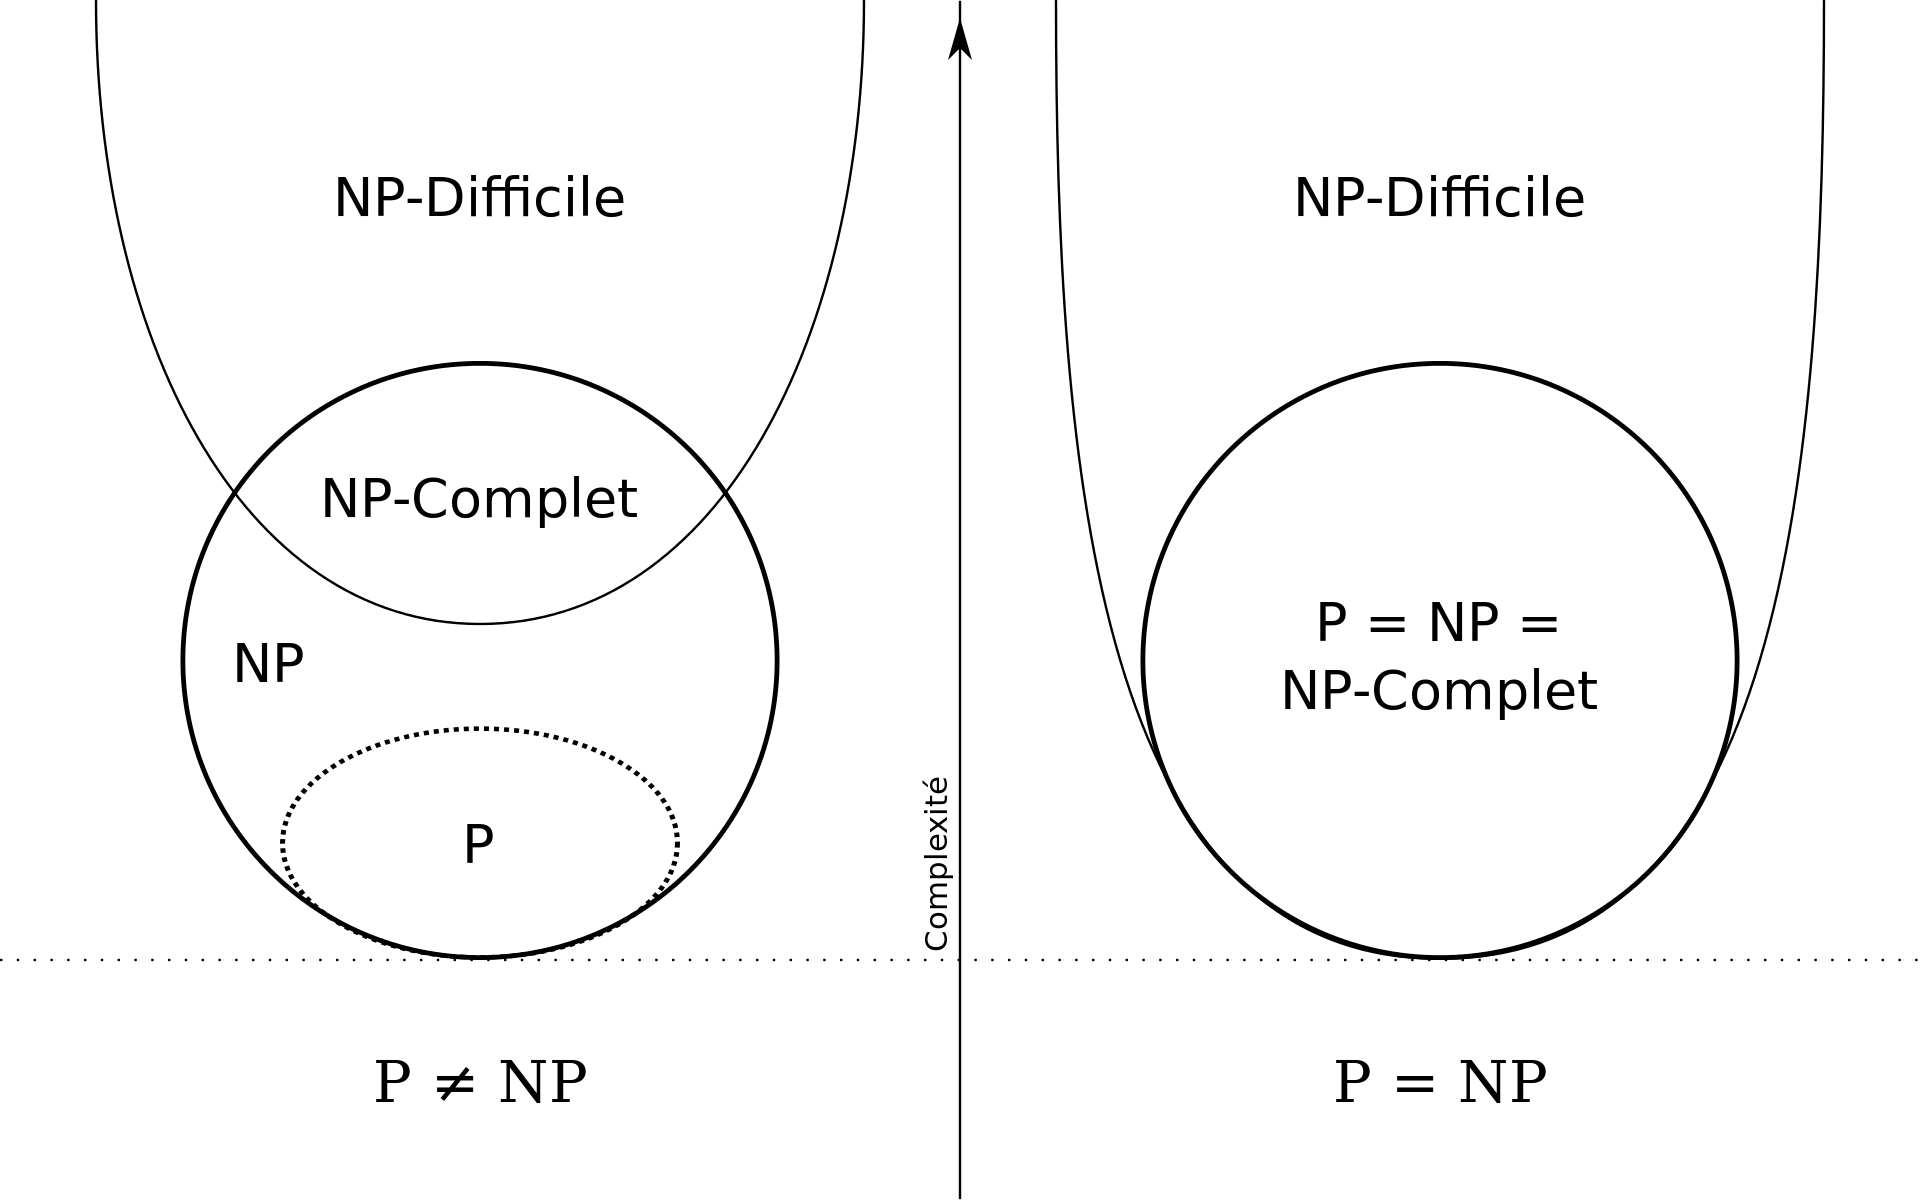
\includegraphics[scale=0.15]{img/pvsnp.png}
	\caption{Illustration des classes de problèmes $\PP$ et $\NP$~\cite{pnp}}
	\label{pnp}
\end{figure}

De manière générale on s'appuie sur les réductions entre problèmes et la caractérisation par certificat de $\NP$ pour montrer qu'un problème donné est $\NPCOMPLETE$. En effet, pour démontrer qu'un problème $A$ est $\NPCOMPLETE$, il suffit de vérifier qu'il est dans $\NP$ via la caractérisation par certificat et de construire une réduction polynomiale d'un problème $B$, que l'on sait être $\NPHARD$, au problème $A$. On peut alors conclure de la façon suivante.

On sait que $\forall C \in \NP, C \leq_P B$ et on a montré $B \leq_P A$, donc $\forall C \in \NP, C \leq_P A$ donc $A$ est $\NPHARD$ et si de plus il est dans $\NP$, il est $\NPCOMPLETE$.

L'un des plus fameux articles sur la question est l'article publié en 1972 par Richard Karp~\cite{21karp}, il propose des réductions pour 21 problèmes de $\NP$ à \textit{SAT}, montrant ainsi que ces $21$ problèmes sont non seulement tous dans $\NP$ mais aussi tous $\NPHARD$ et équivalents entre eux. On parle des $21$ problèmes $\NPCOMPLETE$ de Karp. Plus tard nous verrons une réduction de \emph{min bissection} au problème $max-cut$ qui fait partie des problèmes de Karp.

\subsubsection{P versus NP}

\textit{Digression problème du millénaire...}

Une des grandes questions en informatique fondamentale est de savoir si $\PP = \NP$, si $\PP \not= \NP$ ou si ce résultat est indécidable\ref{pnp}.

Philosophiquement, en se basant sur les définitions de ces deux classes données plus tôt, cela revient à savoir si résoudre un problème en temps polynomial c'est aussi difficile que de vérifier si une solution-candidate est effectivement une solution en temps polynomial. Une analogie, qui donne une bonne idée du problème philosophique est celle avec une preuve de maths. Dans ce cas la question revient à: est-il aussi facile de construire une preuve de maths que de la vérifier une fois construite ? A priori, on a envie de dire qu'il est infiniment plus compliqué de construire une preuve que de vérifier la justesse d'une preuve déjà construite. Néanmoins dans le cas des problèmes en question on n'a pu montrer ni que c'était strictement plus difficile ni que c'était aussi facile. De plus, pour montrer que $\PP = \NP$, il suffirait de fournir un algorithme polynomial pour l'un des problèmes $\NPCOMPLETE$, car tous les problèmes de la classe peuvent se réduire par réduction successive à l'un de ces problèmes en temps polynomial. Cet algorithme serait à même de résoudre tous les problèmes de la classe $\NP$ en temps polynomial.
 
\subsection{Min bissection}

Nous allons travailler avec le problème de décision associé à \textit{min bissection} car le problème d'optimisation n'est a priori pas dans $\NP$ et nous montrerons que ce problème de décision est $\NPCOMPLETE$.

\subsubsection{Appartenance à $\NP$}

\begin{defn}[\textsc{min bissect} -- Problème d'optimisation]
	Soit $G=(V, E)$ un graphe, le problème consiste à trouver $A:B$ une bissection minimale pour $\preceq$ dans $G$.
\end{defn}

\begin{rem}
	C'est en fait une version plus forte du problème de la coupe minimale, dans le cas de la coupe minimale on cherche uniquement une coupe et non une bissection, c'est à dire que les deux communautés n'ont pas à avoir la même taille. Il est important de noter que le problème de la coupe minimale est significativement plus facile à résoudre en terme de complexité algorithmique car il est dans $\PP$. La preuve s'effectue en montrant qu'il y a équivalence entre le problème de la coupe minimale et celui du flot maximum~\cite{papadimitriou1982combinatorial}\footnote{Excellent ouvrage de Christos Papadimitriou, personnage très important en théorie de la complexité et de la théorie des jeux.}, et en vérifiant que ce dernier est soluble en temps polynomial; par exemple avec l'algorithme de Ford-Fulkerson.
\end{rem}

Il n'est a priori pas possible de vérifier que cette bissection est effectivement la plus petite sans la comparer à toutes les bissections possibles. Donc ce problème pas dans $\NP$. Nous allons l'affaiblir de sorte qu'il tombe dans $NP$.

\begin{defn}[Min bissection -- Problème de décision]
	Soient $G=(V, E)$ un graphe et $K \in \N$, le problème consiste à trouver $(A:B)$ une bissection telle que $\card{A:B} < K$.
\end{defn}
Dans ce cas, il est facile de vérifier si l'on a une bissection candidate $A:B$ que $\card{A:B} \leq K$. Il suffit compter le nombre d'arêtes entre les deux ensembles (ou la somme de leur capacité), dans les deux cas, cela se fait en $\Orond(N^2)$ en pire cas. Ainsi le problème de décision de la bissection minimale est  dans $\NP$.

\subsubsection{$\NPHARD$}

La preuve permettant de montrer que \textsc{min-bissection} est $\NPHARD$ se fait grâce à 3 réductions remontant au problème \textsc{3-sat} qui est $NP-complet$ car c'est l'un des 21 problèmes de Karp ~\cite{21karp}. Nous allons montrer successivement:
\[ \text{3-\textsc{sat}} \leq_P \text{\textsc{max-2sat}}\leq_P \text{\textsc{simple-max-cut}} \leq_P \text{\textsc{simple-min-bissect}} \]

Les deux preuves principales sont le passage de \textsc{3-sat} à \textsc{max-2sat} et \textsc{simple-max-cut} à \textsc{simple-min-bissect}, la troisième preuve est plus fastidieuse et peut être omise sans nuire à la compréhension globale, il est néanmoins détaillée dans un souci d'exhaustivité.

\begin{rem}
	Ici nous montrons, en fait, que le problème \textsc{simple-min-bissect}, c'est à dire restreint aux graphes non pondérés reste $\NPHARD$. En effet, il est a priori moins général que \textsc{min-bissect} ie le même problème avec des graphes pondérés. On peut montrer, qu'ils sont en fait équivalent puisque tous deux sont dans $\NPCOMPLETE$ mais la réduction pour le problème générale se fait à partir du problème \textsc{max-cut} dans le cas général.
\end{rem}

\begin{defn}[\textsc{3-sat}~\cite{sat}]
	Soient $C_1 \cdots C_p$ des clauses disjonctives contenant au plus 3 littéraux impliquant des variables $x_1 \cdots x_n$ et $\Phi(x_1 \cdots x_n) =\bigwedge_{i = 1}^p C_i$.
	On dit que $\Phi$ est une formule \textsc{3-sat} et on cherche à décider s'il existe une affectation des variables faisant s'évaluer $\Phi$ à vrai.
\end{defn}

\begin{rem}
	Si on restreint encore le problème \textsc{3-sat} avec des clauses disjonctives contenant au plus deux littéraux on obtient le problème \textsc{2-sat} qui est lui dans $\PP$~\cite{sat}. On voit qu'une restriction en apparence minime change de manière fondamentale la classe de complexité du problème.
\end{rem}

\begin{defn}[\textsc{max-2sat}]
	Soient $C_1 \cdots C_p$ des clauses logiques disjonctives de $2$ littéraux au plus et $K\in \N$ impliquant des variables $x_1 \cdots x_n$. On cherche à décider s'il existe une affectation des variables $(x_i)_i$ telle que $K$ clauses au moins s'évaluent à vrai.
\end{defn}

\begin{defn}[\textsc{simple-max-cut}]
	Soient $G=(V,E)$ et $W \in \N$ on cherche à décider s'il existe une coupe $S_1:S_2$ telle que $\card{S_1:S_2} \geq W$.	
\end{defn}

\begin{defn}[\textsc{simple-min-bissect}]
	Soient $G=(V, E)$ et $W \in \N$, on cherche à décider s'il existe une bissection $\card{A:B} \leq W$.
\end{defn}

\begin{thm}
	 \textsc{3-sat} $\leq_P$ \textsc{max-2sat}.
\end{thm}

\begin{proof}
	Soit $\Irond_1$ une instance de \textsc{3-sat}. Soient $C_1, \cdots C_n$ des clauses disjonctives. On peut supposer sans perte de généralité que toutes ces clauses disjonctives de $\Irond_1$ possèdent exactement 3 littéraux: on peut en effet compléter celles qui en ont moins en ajoutant des variables pour obtenir une formule équivalente et de taille linéaire. On se donne $a_i, b_i, c_i$ pour $i \in [|1, n|]$ les littéraux de la clause $i$. 
	
	\begin{rem}
		Ce ne sont pas des variables distinctes seulement des littéraux c'est à dire une variable ou sa négation. On peut très bien avoir $a_i = b_k = a_j$.
	\end{rem}
	On va construire une instance $\Irond_2$ de \textsc{max-2sat} en formant pour chaque clause $C_i = a_i \lor b_i \lor c_i$ les clauses:
	\begin{enumerate}
		\item $a_i$, $b_i$, $c_i$, $d_i$
		\item $\neg a_i \lor \neg b_i$, $\neg a_i \lor \neg c_i$, $\neg b_i \lor \neg c_i$
		\item $a_i \lor \neg d_i$, $b_i \lor \neg d_i$, $c_i \lor \neg d_i$
	\end{enumerate}

	et on pose $K = 7n$
	
	Cette construction de $\Irond_2$ est linéaire en la taille de $\Irond_1$ et donc a fortiori polynomiale.
	
	Supposons qu'il existe une assignation des variables évaluant la formule \textsc{3-sat} à vrai, alors dans chaque clause, au moins un des littéraux est vrai. On va montrer que quel que soit le nombre de littéraux vrais dans une clause $C_i = a_i \lor b_i \lor c_i$ de $\Irond_1$, il existe une affectation de $d_i$ permettant de valider exactement $7$ clauses dans $\Irond_2$.
	
	Soit $i \in [|1, n|]$, 
		\begin{itemize}
			\item S'il y a un unique littéral à vrai, on suppose sans perte de généralité que c'est $a_i$, alors dans $\Irond_2$: $(a_i), (\neg a_i \lor \neg b_i), (\neg a_i \lor \neg c_i), (\neg b_i \lor \neg c_i)$ sont vraies, et quitte à prendre $d_i=\bot$ on a  $(a_i \lor \neg d_i)$, $(b_i \lor \neg d_i)$, $(c_i \lor \neg d_i)$ vraies aussi. On a alors $7$ clauses vraies.
			\item S'il y a exactement 2 littéraux à vrai, on suppose sans perte de généralité que c'est $a_i, b_i$ alors dans $\Irond_2$: $(a_i), (b_i), (\neg a_i \lor \neg c_i), (\neg b_i \lor \neg c_i)$ sont vraies et quitte à prendre $d_i=\bot$ on a aussi $(a_i \lor \neg d_i)$, $(b_i \lor \neg d_i)$, $(c_i \lor \neg d_i)$ vraies. Et donc bien exactement 7 clauses vraies.
			\item Si les 3 littéraux sont vrais, alors dans ce cas dans $\Irond_2$: $(a_i), (b_i), (c_i), (a_i \lor \neg d_i)$, $(b_i \lor \neg d_i)$, $(c_i \lor \neg d_i)$ sont vraies et quitte à prendre $d_i=\top$ $(d_i)$ aussi est vrai et on a bien nos $7$ clauses.
		\end{itemize}
	
	On note que dans chacun des cas, l'autre affectation de $d$ donne strictement moins de $7$ clauses vraies.
	
	Ainsi si $\Irond_1$ possède une solution alors $\Irond_2$ possède également une solution.
	
	On montre maintenant que si $\Irond_2$ possède une solution alors $\Irond_1$ en possède une aussi. Par contraposée, on suppose qu'il n'existe pas d'affectation évaluant la formule \textsc{3-sat} à vrai. Ainsi, il existe au moins une clause dont aucun des littéraux n'est vrai. Dans ce cas, on vérifie qu'au plus $6$ clauses (pour $d_i = \bot$) peuvent être vérifiées, ainsi il y a strictement moins de $7m$ clauses vérifiées dans $\Irond_2$.
	
	Ainsi $\Irond_1$ a une solution si et seulement si $\Irond_2$ a une solution. On a donc bien montré que \textsc{3-sat} se réduit à \textsc{max-2sat}	
\end{proof}

\begin{thm}
	$\textsc{max-2sat} \leq_\textsc{P simple-max-cut}$.
\end{thm}

\begin{proof}
	Soit $\Irond_1$ une instance de \textsc{max-2sat} nous allons construire une instance $\Irond_2$ de \textsc{simple-max-cut}.
	
	Soient $C_1 \cdots C_m$ les clauses de $\Irond_1$ et $K$ le nombre de clauses à valider, on peut supposer qu'elles contiennent toutes exactement $2$ littéraux, quitte à répéter le littéral présent dans la clause, pour obtenir une formule équivalente.
	
	Dans ce cas pour tout $i \in [|1, m|]$ on note $C_i = a_i \cup b_i$. On note $x_1 \cdots x_n$ les variables (et leur négation) impliquées dans les clauses de $\Irond_1$. On construit alors un graphe  $G=(V,E)$ de \textsc{simple-max-cut}.
	
	On forme $V$ les sommets du graphe de la façon suivante:
	\begin{align*}
		V = \set{T_i : 0 \leq i \leq 3m} &\cup \set{F_i : 0 \leq i \leq 3m} \cup \set{t_{ij} : 1 \leq i \leq n, 0\leq j \leq 3m} \\ &\cup \set{f_{ij} : 1 \leq i \leq n, 0\leq j \leq 3m} \\
			&\cup\set{x_i : 1 \leq i \leq n} \\
			&\cup\set{\bar{x_i} : 1 \leq i \leq n}
	\end{align*}
	On commence par construire un premier ensemble d'arêtes:	
	\begin{align*}
		A_1 &= \set{(T_i, Fj) : 0 \leq i \leq 3m, 0 \leq j \leq 3m } \\
			&\cup \set{(t_{ij}, f_{ij}), 0 \leq i \leq n, 0 \leq j \leq 3m} \\
			&\cup \set{(x_i, f_{ij}), 0 \leq i \leq n, 0 \leq j \leq 3m} \\
			&\cup \set{(\bar{x_i}, t_{ij}), 0 \leq i \leq n, 0 \leq j \leq 3m} \\
			\\
		A_2 &= \set{(a_i,b_i): 0 \leq i \leq m, a_i \not= b_i} \cup \set{(a_i, F_{2i-1}) : 0 \leq i \leq m} \\
			&\cup \set{(b_i, F_{2i}) : 0 \leq i \leq m}
	\end{align*}
	
	Dans la suite on dit, soit une partition $S_1, S_2$ des sommets que $(u, v)$ est une bonne arête si et seulement si $u$ et $v$ appartiennent au même ensemble de la partition et que c'est une mauvaise arête sinon. On fait tout d'abord remarquer que toutes les arêtes de $A_1$ dès qu'une partition vérifie que tous les $T_i$ sont dans un même ensemble et tous les $F_i$ dans l'autre et si pour tout $i$, $x_i$ et les $f_{ij}$ sont dans un même ensemble et $\bar{x_i}$ et tous les $t_{ij}$ dans l'autre.
	
	De plus, si on a $F_i, F_j$, $i \not= j$ dans deux ensembles différents alors on a au moins $3m+1$ arêtes de $A_1$ qui seront mauvaises (ie avec une extrémité dans un ensemble de la partition et l'autre dans l'autre) puisque ces deux sommets ont en commun $3p+1$ voisins communs. De même, on a que si $x_i, \bar{x_i}$  sont dans le même ensemble, alors de la partition au moins $3m+1$ arêtes de $A_1$ seront mauvaises car il y a $3m+1$ chemin (disjoints) de longueur 3 de $x_i$ à $\bar{x_i}$.
	
	
	On construit ainsi $G=(V, E=A_1 \cup A_2)$ et $W = \card{A_1} + 2K$ une instance $\Irond_2$ de \textsc{simple-max-cut}.
	
	On suppose que $\Irond_1$ possède une solution, c'est à dire un assignement des variables $x_1 \cdots x_n$ rendant au moins $K$ clauses vraies.
	
	On construit alors une partition $S_1, S_2$ des sommets de $G$:
	
	\begin{align*}
		S_1 &= \set{(T_i, Fj) : 0 \leq i \leq 3m, 0 \leq j \leq 3m }
		\cup \set{x_i : x_i = \bot} \\
		&\cup \set{t_{ij} : x_i = \bot, 0 \leq j \leq 3m } \\
		&\cup \set{\bar{x_i}, x_i = \top} \\
		&\cup\set{f_{ij}, x_i = \top,  0 \leq j \leq 3m} \\ \\
		S_2 &= V \backslash S_1
	\end{align*}
	
	Chaque clause possède alors un ou deux littéraux évalués à vrai et donc $a_i$ ou $b_i$ appartient à $S_2$ or dans $A_2$ il y a exactement $2$ arêtes tombant sur cette clause qui sont bonnes. De plus toutes les arrêtes de $A_1$ sont donc bonnes. Et on a bien $W = \card{A_1} + 2k$.
	
	Réciproquement, si on a $S_1', S_2'$ une partition dont au moins $W$ arêtes sont bonnes on a $\card{A_2} \leq 3m$ et $K \geq 0$. On en déduit qu'on a au plus $3m$ mauvaises arêtes.
	
	Cela implique que tous les $F_i$ sont dans le même ensemble de la partition, disons $S_1'$, on a aussi pour chaque paire $x_i, \bar{x_i}$ l'un des deux appartient à $S_1'$.
	
	Il suffit alors d'assigner la valeur $\top$ à $x_i$ si et seulement si il appartient à $S_2'$.
	
	\begin{exercice}
		Le lecteur consciencieux pourra vérifier que cet assignement garantit qu'au moins $K$ clauses de $\Irond_1$ sont vérifiées.
	\end{exercice}
\end{proof}
\begin{thm}
	$\textsc{simple-max-cut} \leq_P \textsc{simple-min-bissect}$
\end{thm}

\begin{proof}
Soit $\Irond_1$ une instance du problème \textsc{simple-max-cut}, soit $G=(V,E)$ et $W \in \N^*$. On va construire une instance $\Irond_2$ de \textsc{MIN-BISSECTION}, on note $N = \card{V}$.

On construit $V' = V \cup \set{U_1 \cdots U_N}$ avec $\set{U_1 \cdots U_N} \cap V = \emptyset$. On double en fait le nombre de sommets par rapport au graphe initial pour garantir que l'on ait un nombre pair de sommets et pour ainsi pouvoir former la partition en ensembles de tailles égales.

On relie alors dans $G'$ uniquement les sommets qui ne sont pas reliés dans $G$ (les sommets ajoutés forment une clique) ie $E' = \set{(u,v) : u,v \in V', (u,v) \not \in E}$. Et on fixe $W' = N^2 - W$.

Supposons alors que $\Irond_1$ possède une coupe solution: $S_1:S_2$ telle que $\card{S_1:S_2} \geq W \geq 1$, on a $S_1$ et $S_2$ non vides.
On complète $S_1$ et $S_2$ avec les sommets $U_i$ de sorte à former $S_1'$ et $S_2'$ de même taille.

On va vérifier que $S_1':S_2'$ forme une bissection de poids plus petit que $W'$
\begin{align*}
	\card{S_1':S_2'} = N^2 - \card{\set{(u,v) \not \in E' : u \in S_1', v \in S_2'}} &= N^2 - \card{\set{(u,v) \in E : u \in S_1, v \in S_2}} \\
					& \leq N^2 - W = W'
\end{align*}
Ainsi si $\Irond_1$ a une solution alors $\Irond_2$ a une solution. Montrons maintenant la réciproque.

Supposons que $\Irond_2$ ait une solution $\card{S_1':S_2'} \leq W' = N^2 - W$. On définit alors $S_1 = S_1' \cap V$ et $S_2 = S_2' \cap V$. On va voir que $S_1:S_2$ est une solution de $\Irond_1$.

En effet: 
\begin{align*}
	\card{S_1:S_2} = \card{\set{(u,v) \not \in E' : u \in S_1', v \in S_2'}} &= N^2 -  \card{\set{(u,v) \in E' : u \in S_1', v \in S_2'}} \\
				   &\geq N^2 - (N^2 - W) = W
\end{align*}
Ainsi si $\Irond_2$ a une solution alors $\Irond_1$ a une solution.

De plus la construction présentée est polynomiale en la taille du problème, donc c'est une réduction polynomiale. On conclut donc que tout problème de \textsc{simple-max-cut} peut être transformé en un problème équivalent de \textsc{simple-min-bissect} qui est donc $\NPHARD$. 
\end{proof}

On a alors montré que le problème de décision de la bissection minimale était bien $\NP$ et $\NPHARD$, il est donc bien $\NPCOMPLETE$.
\end{document}
